\documentclass[10pt,unknownkeysallowed]{beamer}

\usetheme[progressbar=frametitle]{metropolis}
\usepackage{appendixnumberbeamer}
\usepackage{graphicx}
\usepackage{booktabs}
\usepackage[scale=2]{ccicons}

\usepackage{pgfplots}
\usepgfplotslibrary{dateplot}

\usepackage{xspace}
\newcommand{\themename}{\textbf{\textsc{metropolis}}\xspace}
\newcommand{\mat}[1]{\mbox{\boldmath{$#1$}}} 
\title{Spatial Autoregressive Models within GAMLSS}
\subtitle{Master Thesis}
% \date{\today}
\date{25/07/2019}
\author{Lucas de Miranda Oliveira}
\institute{UFPE}
% \titlegraphic{\hfill\includegraphics[height=1.5cm]{logo.pdf}}

\begin{document}

\maketitle

\begin{frame}{Outline}
  \setbeamertemplate{section in toc}[sections numbered]
  \tableofcontents[hideallsubsections]
\end{frame}

\section{Introduction}


\section{Elements}
\section{Simulations Studies}


\begin{frame}{Simulation study I}

We generate $n$ polygons through the \textit{Voronoi Diagram}, in which the points are generated randomly in a square area. The Voronoi Diagram subdivides the space into cells as shown in figure below, which displays 50 regions generated. The \texttt{voronoi.polygons}() function of the \textbf{SDraw} package implemented in the \texttt{R} software was used to generate the areas.
\vspace{-2.5cm}
 \begin{figure}
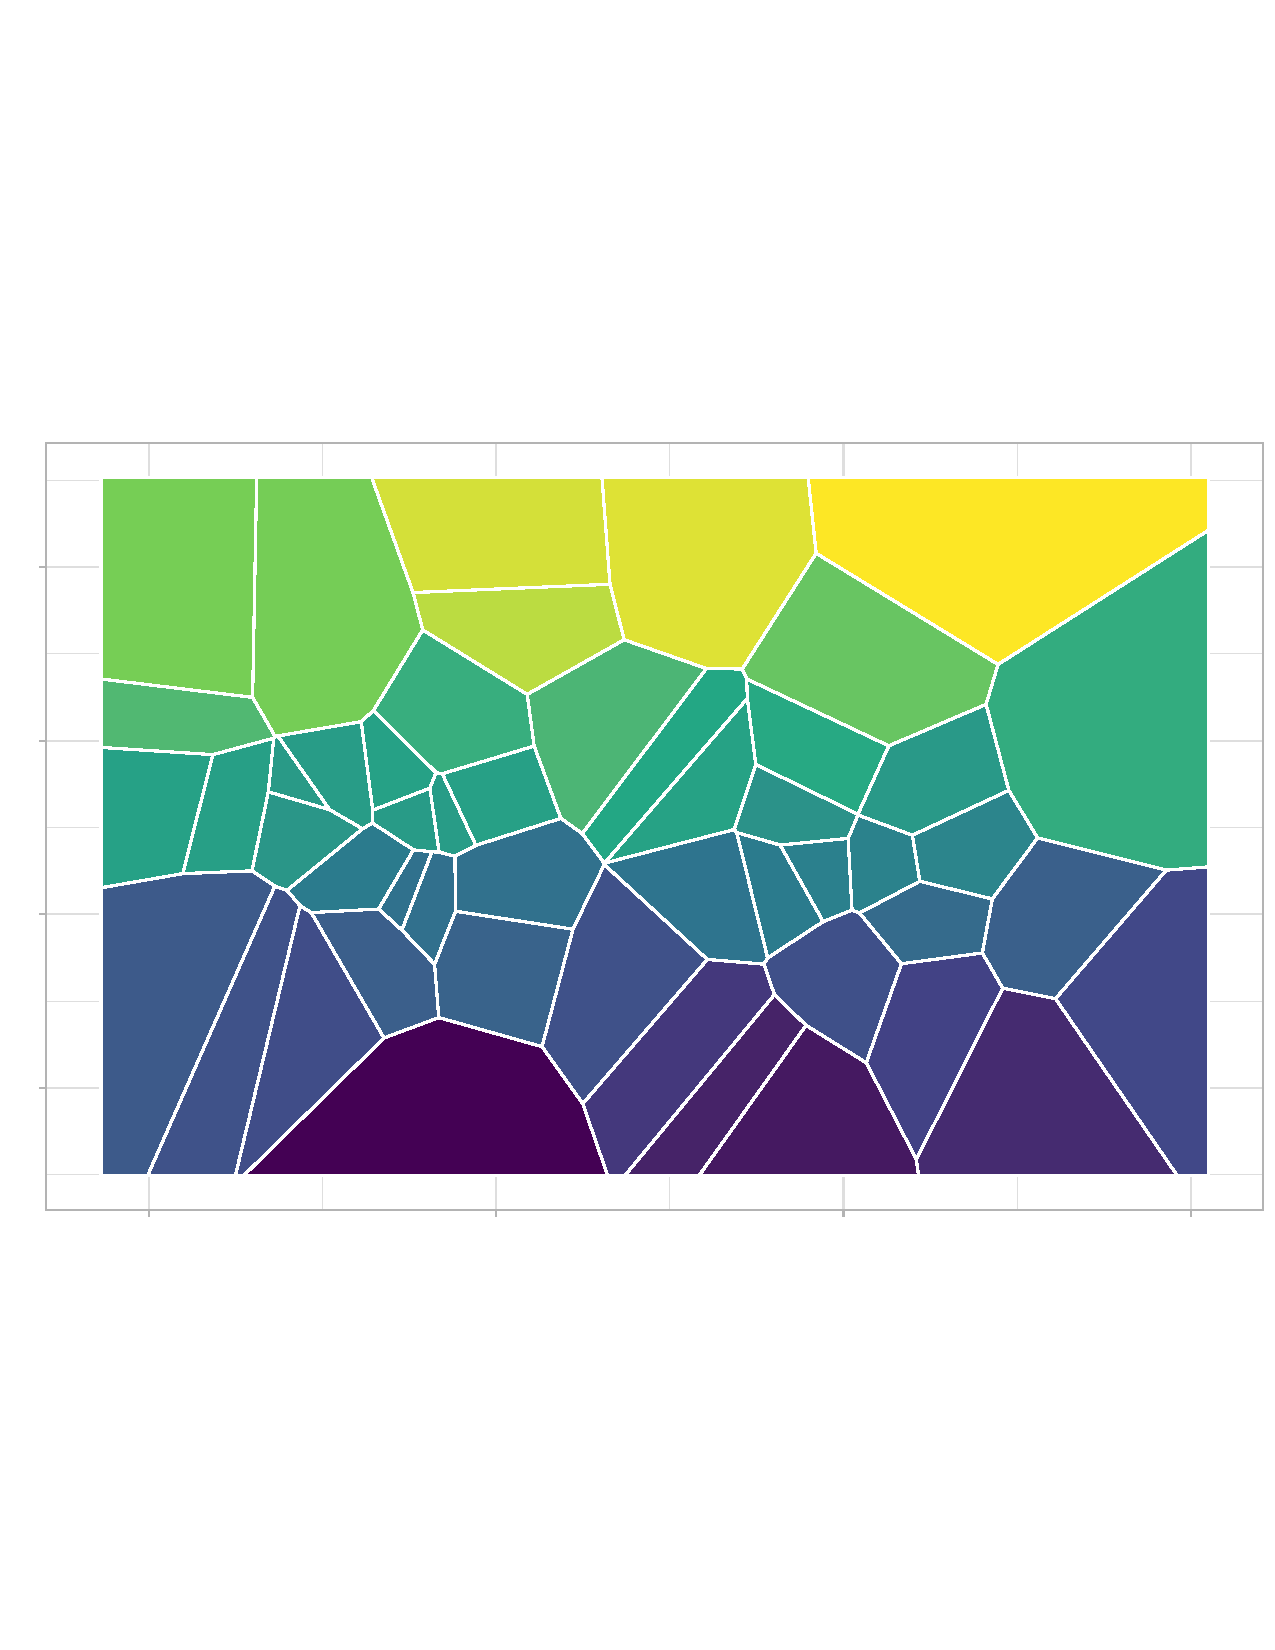
\includegraphics[width=0.7\linewidth]{VoroniDiagrams.pdf}
\label{fig:Voronoi Partition}
\caption{\textit{Voronoi Diagram}}
\end{figure}
\end{frame}

\begin{frame}{Simulation design}
In order to evaluate the finite sample properties of the estimators of the coefficients  for proposed model,
 we calculated the bias and MSE and of the estimator and compute AIC,  considering simulations
with sample size varying as n = 20, 40 and 60. These quantities were calculated using the following formulas:

\begin{align*}
   \textrm{RB-E}&=\frac{1}{m}\sum_{i=1}^{m}\frac{\hat{\beta}_k^{(i)}-\beta_k}{\beta_k}, \nonumber \\
     \textrm{MSE-E}&= \frac{1}{m}\sum_{i=1}^{m}(\hat{\beta}_k^{(i)}-\beta_k)^2, \\
      \textrm{AIC-E}&=\frac{1}{m}\sum_{i=1}^{m}-2l(\hat{\theta})^{(i)}+2j
      \end{align*}




\end{frame}

\begin{frame}{Simulation design}
Based on Haining (2003) the simulation study was performed as follows:
 \begin{itemize}
    \item Obtain the cholesky decomposition for a square matrix $\mat{\Sigma}$ of order $n$ such that $\mat{\Sigma}= \textbf{\textrm{L}}\textbf{\textrm{L}}^\top$.  Where $\textbf{\textrm{L}}$ is a lower triangular n by n matrix. The valid matrix taken here is the covariance matrix of the SAR model;
    
    \item Generate the $n$ observations of the covariates  $\underline{\mat{x}}_1$ and $\underline{\mat{x}}_1$ that follows from a uniform ($\mathcal{U}$) probability distribution in the range of 0 to 3;

    \item  For each of the 1000 replicates of monte carlo a vector $\underline{\mat{\varepsilon}}$ of length $n$ is generated from uncorrelated normal random variables; and
    
    \item  Compute response variable $\underline{\mathbf{y}}$ with spatial dependency for each replicate by doing $\underline{\mat{y}}= \mat{\mu} + \textbf{\textrm{L}}\underline{\mat{\varepsilon}}$ , where $\underline{\mat{\mu}} = \beta_0 +\beta_1 \underline{\mat{x}}_1+\beta_2 \underline{\mat{x}}_2$.
    \end{itemize}
\end{frame}

\begin{frame}{Simulation design}
 The true values of the parameters are  $(\beta_0,\beta_1,\beta_2)=(2.5,0.5,0.2)$, $\rho=(0,0.1)$, and $\sigma=1$. 
 We compared regression coefficients estimators of linear model (LM), without spatial dependence, \textit{lag} spatial (L-SAR) model and SAR incorporated into the GAMLSS (SAR-GAMLSS). The first LM and L-SAR are given, respectively, by:

     \begin{align*}
      \underline{\mat{y}}&= \beta_0+\beta_1\underline{\mat{x}}_1+\beta_2\underline{\mat{x}}_2
    + \underline{\mat{\varepsilon}}, \nonumber \\
    \underline{\mat{y}}&= \beta_0+ \beta_1\underline{\mat{x}}_1+\beta_2\underline{\mat{x}}_2+
    \rho \textbf{\textrm{W}} \underline{\mat{y}}+\underline{\mat{\varepsilon}}, \nonumber \\
     \end{align*}

 \noindent with $\mat{\varepsilon}\sim \textrm{N}(\mat{0},\sigma^2\textbf{\textrm{I}})$ the same for the two models, and $\textbf{\textrm{x}}_1$ is the fixed  covariate generated.
\end{frame}


\begin{frame}{Results}
    
\end{frame}

\begin{frame}{Simulation based on Boston Housing \textit{data}}

Hedonic pricing data of Harrison and Rubinfeld (1978), in its corrected version (Gilley and Pace, 1996). In this article, the authors analyzed the demand for clean air through a hedonic price model for residences in Boston.

The variables are:
\begin{itemize}
    \item \texttt{PRICE}: logarithm of the median corrected value of household values in USD 1000's;
    \item \texttt{CRIM}: crime per capita in the town;
    \item \texttt{AGE}: the units occupied by the owners, proportionally, which were built before the year 1940;
    \item \texttt{NOX}: nitrogen oxides concentration;
    \item \texttt{RM}: average number of rooms per dwelling;
    \item  \texttt{ZN}: proportion of residential land zoned for lots over 25,000;
    \item  \texttt{INDUS}: proportion of non-retail business acres per town;
    \item \texttt{TAX}: full-value property-tax rate per 10,000;
    \end{itemize}
    \end{frame}
    
    \begin{frame}{Simulation based on Boston Housing \textit{data}}
    \begin{itemize}
    \item \texttt{PTRATIO}: pupil-teacher ratio by town; 
    \item \texttt{RAD}: index of accessibility to radial highways;
        \item \texttt{B}: $1000*(\textrm{Bk} - 0.63)^2$, where Bk is the proportion of blacks by town;
   \item \texttt{LSTAT}: lower status of the population; and
   \item \texttt{DIS}: weighted mean of distances to five Boston employment centres 
    \end{itemize}
\end{frame}

\begin{frame}{ Simulation design}
The simulation study based on real \textit{data} was performed as follows:
\begin{enumerate}
   \item Cholesky decomposition was computed for a SAR covariance matrix $\mat{\Sigma}$ of order $n=506$, where each $n$ corresponds to census tracts  in the Boston Housing \textit{data}, and  the true value of spatial correlation parameter was $\rho=0.10$;
    \item  For each of the 1000 replicates of Monte Carlo a vector $\underline{\mat{\varepsilon}}$ of length $n$ is generated from uncorrelated normal random variables; and
    \item  Compute response variable $\underline{\mathbf{y}}$ with spatial dependency for each replicate by doing $\underline{\mat{y}}= \mat{\mu} + \textbf{\textrm{L}}\underline{\mat{\varepsilon}}$, where $\underline{\mat{\mu}} = \beta_0+ \beta_1\texttt{RM} + \beta_2\texttt{RAD}$, and $\textrm{Y}\sim \textrm{ Sinh-Arcsinh}(\mu,\sigma=1,\nu=0.5)$. The true values for $\underline{\beta}$ are
    $\underline{\beta}=(\beta_0,\beta_1,\beta_2)=(1,0.5,0.5)$.
\end{enumerate}
\end{frame}

\begin{frame}{Results}
Figure \ref{fig:BostonBox} shows boxplots for estimates of parameters of regression.
\center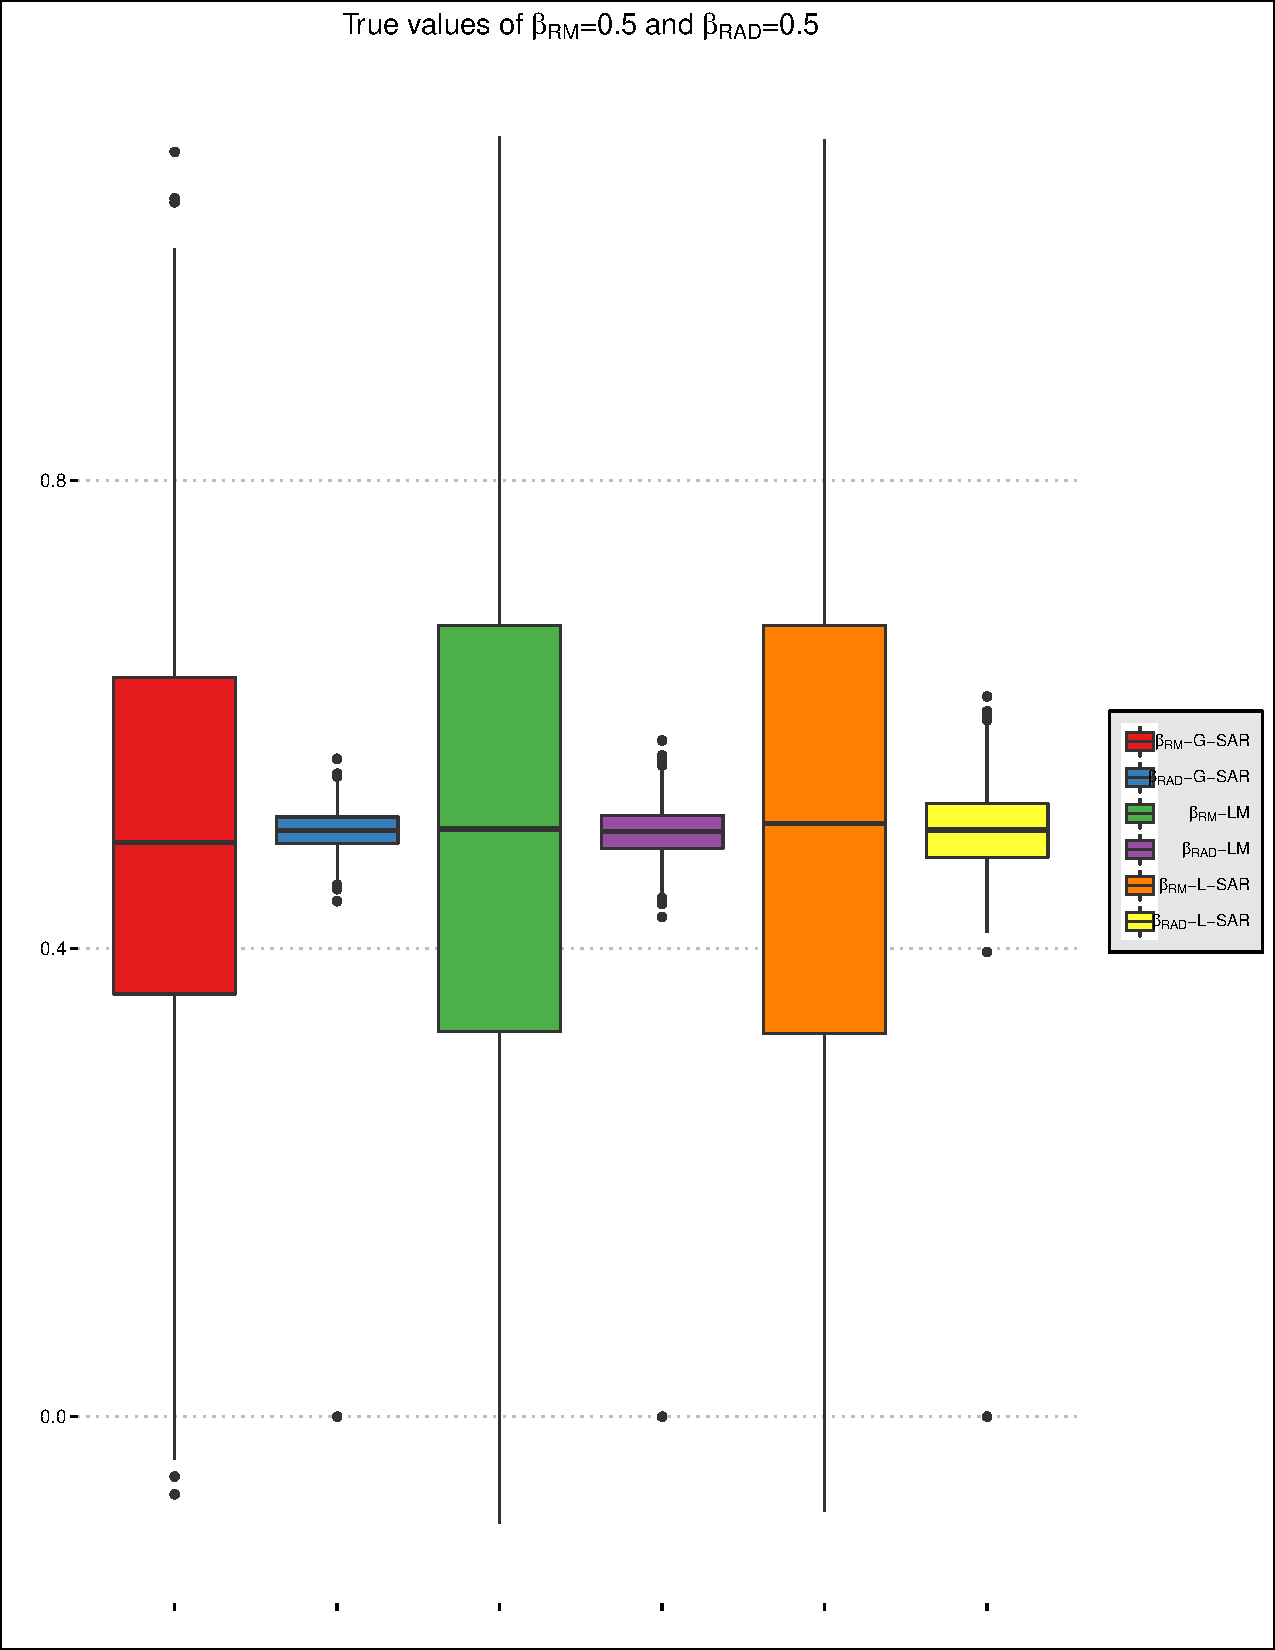
\includegraphics[width=4cm,height=5cm]{Betas_Boston_boxplot.pdf}\label{fig:BostonBox}
\end{frame}

\begin{frame}{Results}
\begin{table}[]
\begin{tabular}{ccc}
\hline
LM       & L-SAR    & G-SAR             \\ \hline
2872.469 & 2873.453 & \textbf{2764.275} \\ \hline
\end{tabular}
\caption{Empirical AIC for models}
\end{table}
\end{frame}

\section{Applications}



\section{Conclusion}

{\setbeamercolor{palette primary}{fg=black, bg=yellow}
\begin{frame}[standout]
  Questions?
\end{frame}
}


\begin{frame}[allowframebreaks]{References}

  \bibliography{demo}
  \bibliographystyle{abbrv}

\end{frame}

\end{document}